\chapter{CƠ SỞ LÝ THUYẾT VÀ CÁC NGHIÊN CỨU LIÊN QUAN}

Trong chương này, luận văn trình bày nền tảng lý thuyết cần thiết để làm rõ bối cảnh và nội dung của bài toán nghiên cứu. Trước hết, chương giới thiệu các khái niệm về tín dụng, rủi ro tín dụng, phân loại nhóm nợ và tổn thất kỳ vọng. Tiếp theo, chương phân tích sự chuyển dịch từ phương pháp đánh giá truyền thống sang các mô hình học máy, trong đó tập trung vào các thuật toán được sử dụng trong phần thực nghiệm. Những thách thức đặc thù của dữ liệu tín dụng, bao gồm mất cân bằng lớp, tính thứ tự của nhóm nợ, sự thay đổi phân bố theo thời gian và yêu cầu giải thích mô hình, cũng được thảo luận. Cuối cùng, chương trình bày hệ thống chỉ tiêu đánh giá, tổng quan các nghiên cứu liên quan và xác định khoảng trống mà luận văn hướng tới giải quyết. Đây là cơ sở lý luận để xây dựng quy trình nghiên cứu ở Chương 3.

\section{Nền tảng tín dụng, rủi ro và phân loại nhóm nợ}

\subsection{Khái niệm tín dụng và rủi ro tín dụng}

Tín dụng là quan hệ kinh tế trong đó bên cho vay chuyển giao quyền sử dụng một lượng giá trị cho bên đi vay trong một khoảng thời gian xác định, với nghĩa vụ hoàn trả theo các điều kiện đã thỏa thuận.

Rủi ro tín dụng là khả năng phát sinh tổn thất do khách hàng hoặc đối tác không thực hiện đầy đủ nghĩa vụ tài chính. Rủi ro chịu ảnh hưởng từ năng lực tài chính, đặc điểm khoản vay, lịch sử tín dụng, chính sách cấp tín dụng và điều kiện kinh tế.

\subsection{Phân loại nhóm nợ}

\begin{table}[H]
\centering
\caption{Các nhóm nợ trong nghiên cứu}
\begin{tabular}{|c|p{4cm}|p{7cm}|}
\hline
1 & Nợ đủ tiêu chuẩn & Mức rủi ro thấp.\\
\hline
2 & Nợ cần chú ý & Đã xuất hiện dấu hiệu cần theo dõi.\\
\hline
3 & Nợ dưới tiêu chuẩn & Khả năng thu hồi suy giảm đáng kể.\\
\hline
4 & Nợ nghi ngờ & Mức rủi ro cao.\\
\hline
5 & Nợ có khả năng mất vốn & Mức rủi ro cao nhất.\\
\hline
\end{tabular}
\end{table}

\subsection{Xếp hạng tín dụng và tổn thất kỳ vọng}

Xếp hạng tín dụng là quá trình gán khách hàng hoặc khoản vay vào một hạng rủi ro dựa trên thông tin tài chính, đặc điểm khoản vay và lịch sử thực hiện nghĩa vụ. Trong phạm vi luận văn, năm nhóm nợ được xem là các mức rủi ro có thứ tự; mô hình được xây dựng để hỗ trợ nhận diện nhóm nợ tương ứng của từng quan sát.

Tổn thất kỳ vọng có thể biểu diễn:
\[
EL=PD\times LGD\times EAD.
\]
Trong đó $EL$ là tổn thất kỳ vọng; $PD$ là xác suất vỡ nợ trong kỳ đánh giá; $LGD$ là tỷ lệ tổn thất khi vỡ nợ sau khi xét khả năng thu hồi; và $EAD$ là dư nợ tại thời điểm vỡ nợ. Luận văn hiện tập trung vào phân loại trạng thái rủi ro, chưa trực tiếp ước lượng đủ ba cấu phần của $EL$ \cite{basel_framework}.

\begin{figure}[H]
\centering
\begin{tikzpicture}[
    >=stealth,
    font=\small,
    riskbox/.style={draw, rounded corners=2pt, align=center, minimum height=1.8cm, text width=3.7cm},
    resultbox/.style={draw, rounded corners=2pt, very thick, align=center, minimum height=1.45cm, text width=4.2cm}
]
    \node[riskbox] (pd) at (-5.0,1.6)
        {\textbf{$PD$}\\Xác suất khách hàng vỡ nợ trong kỳ đánh giá};
    \node[riskbox] (lgd) at (0,1.6)
        {\textbf{$LGD$}\\Tỷ lệ tổn thất sau khi xét phần có thể thu hồi};
    \node[riskbox] (ead) at (5.0,1.6)
        {\textbf{$EAD$}\\Dư nợ của khoản cấp tín dụng tại thời điểm vỡ nợ};
    \node[resultbox] (el) at (0,-1.25)
        {\textbf{Tổn thất kỳ vọng}\\$EL=PD\times LGD\times EAD$};
    \draw[->, very thick] (pd.south) -- (el.north west);
    \draw[->, very thick] (lgd.south) -- (el.north);
    \draw[->, very thick] (ead.south) -- (el.north east);
\end{tikzpicture}
\caption{Các cấu phần của tổn thất kỳ vọng trong rủi ro tín dụng}
\label{fig:el-components}
\caption*{\textit{Nguồn: Tác giả tổng hợp và vẽ lại từ Basel Committee on Banking Supervision \cite{basel_framework}.}}
\end{figure}

\section{Từ đánh giá truyền thống đến các mô hình học máy}

\subsection{Sự chuyển dịch từ phương pháp truyền thống sang học máy}

Phương pháp chuyên gia có khả năng khai thác thông tin định tính nhưng chủ quan. Z-score của Altman có ý nghĩa nền tảng nhưng phụ thuộc dữ liệu kế toán và quan hệ tuyến tính. Logistic Regression dễ giải thích nhưng khó tự động nắm bắt tương tác phức tạp.

Học máy là nhánh của AI trong đó mô hình học quy luật từ dữ liệu. Bài toán của luận văn thuộc học có giám sát.

\subsection{Mô hình tuyến tính và cây quyết định}

\noindent\textbf{Logistic Regression đa lớp.}

\[
P(Y=k\mid\mathbf{x})
=
\frac{\exp(\beta_{k0}+\boldsymbol{\beta}_{k}^{T}\mathbf{x})}
{\sum_{j=1}^{K}\exp(\beta_{j0}+\boldsymbol{\beta}_{j}^{T}\mathbf{x})}.
\]
Trong đó $K$ là số lớp; $\mathbf{x}$ là véc-tơ đặc trưng; $\beta_{k0}$ là hệ số chặn của lớp $k$; $\boldsymbol{\beta}_{k}$ là véc-tơ hệ số của lớp $k$; và mẫu số chuẩn hóa để tổng xác suất của $K$ lớp bằng 1 \cite{hosmer2013applied}.

\medskip
\noindent\textbf{Decision Tree.}

Decision Tree chia không gian đặc trưng bằng các điều kiện dạng $x_j\le s$. Mô hình dễ giải thích nhưng dễ overfitting.

\medskip
\noindent\textbf{Random Forest.}

\[
\hat{y}=\operatorname{mode}\{h_b(\mathbf{x})\}_{b=1}^{B}.
\]
Trong đó $B$ là số cây; $h_b(\mathbf{x})$ là dự báo lớp của cây thứ $b$ tại hồ sơ $\mathbf{x}$; và $\operatorname{mode}$ chọn lớp xuất hiện nhiều nhất trong các dự báo cây \cite{breiman2001random}.

\subsection{Các mô hình boosting}

\noindent\textbf{XGBoost.}

\[
\mathcal{L}^{(t)}
=
\sum_{i=1}^{n}
l(y_i,\hat{y}_{i}^{(t-1)}+f_t(\mathbf{x}_i))
+\Omega(f_t).
\]
Trong đó $t$ là vòng boosting; $n$ là số quan sát huấn luyện; $l(\cdot)$ là hàm mất mát; $\hat{y}_{i}^{(t-1)}$ là dự báo tích lũy trước vòng $t$; $f_t$ là cây mới; và $\Omega(f_t)$ là số hạng phạt độ phức tạp của cây nhằm hạn chế quá khớp \cite{chen2016xgboost}.

\begin{figure}[H]
\centering
\begin{minipage}{0.46\textwidth}
    \centering
    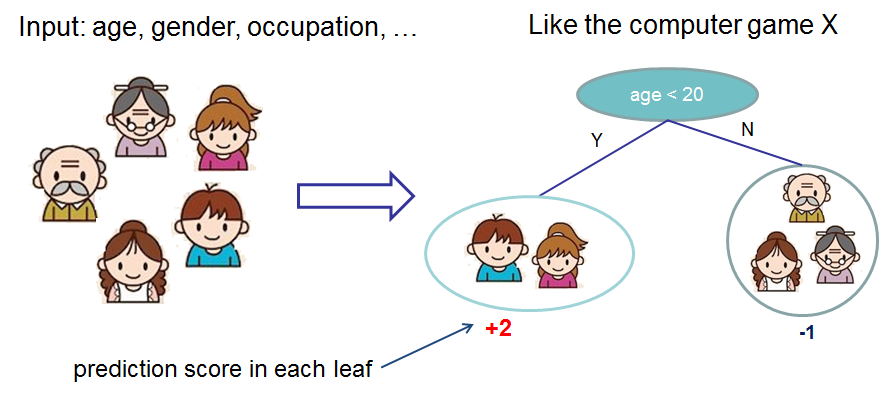
\includegraphics[width=\linewidth]{figures/xgboost_cart_example.png}
    \\[1mm]\small (a) Một cây CART đơn — mỗi hồ sơ nhận điểm dự báo tại lá tương ứng
\end{minipage}
\hfill
\begin{minipage}{0.5\textwidth}
    \centering
    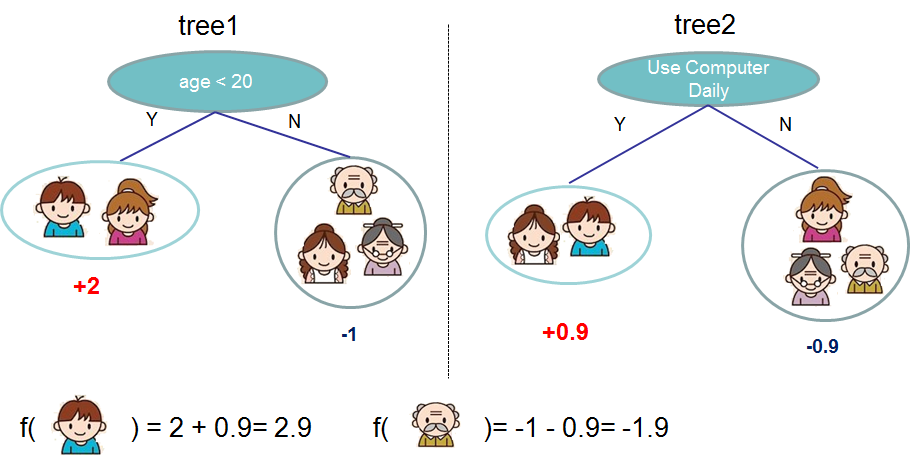
\includegraphics[width=\linewidth]{figures/xgboost_two_trees.png}
    \\[1mm]\small (b) Cộng dồn điểm dự báo của nhiều cây: $f(\mathbf{x})=\sum_t f_t(\mathbf{x})$
\end{minipage}
\caption{Cơ chế cộng dồn các cây trong XGBoost}
\label{fig:xgboost-additive}
\caption*{\textit{Nguồn: Tài liệu chính thức của XGBoost \cite{xgboost_docs}, giấy phép Apache 2.0; minh họa cho cơ chế mô tả trong Chen và Guestrin \cite{chen2016xgboost}; truy cập ngày 15/08/2026.}}
\end{figure}

Hình~\ref{fig:xgboost-additive} thể hiện cách dự báo được cập nhật tuần tự. Mỗi cây mới $f_t(\mathbf{x})$ hiệu chỉnh phần sai số còn lại của tổ hợp trước đó bằng cách cộng thêm điểm số tại lá tương ứng của hồ sơ đang xét, có nhân hệ số học $\eta$; XGBoost đồng thời đưa số hạng chính quy $\Omega(f_t)$ vào hàm mục tiêu để kiểm soát độ phức tạp.

\medskip
\noindent\textbf{LightGBM.}

LightGBM tối ưu tốc độ và bộ nhớ bằng các kỹ thuật như Gradient-based One-Side Sampling và Exclusive Feature Bundling. Thuật toán phát triển cây theo lá tốt nhất, tức là tại mỗi bước ưu tiên tách lá tạo ra mức giảm hàm mất mát lớn nhất. Cách phát triển này có thể hội tụ nhanh nhưng cũng làm cây mất cân đối và dễ quá khớp khi dữ liệu nhỏ; vì vậy cần kiểm soát \mbox{\texttt{num\_leaves}}, \mbox{\texttt{min\_data\_in\_leaf}} và \mbox{\texttt{max\_depth}} \cite{ke2017lightgbm,lightgbm_docs}.

\begin{figure}[H]
\centering
\begin{minipage}{0.48\textwidth}
    \centering
    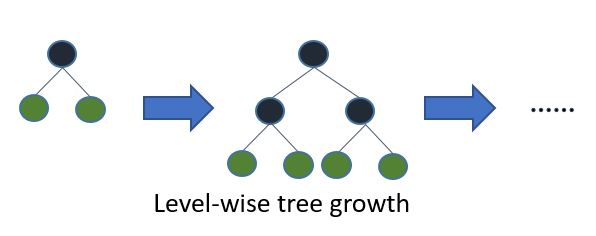
\includegraphics[width=\linewidth]{figures/lightgbm_level_wise.png}
    \\[1mm]\small (a) Phát triển cây theo tầng
\end{minipage}
\hfill
\begin{minipage}{0.48\textwidth}
    \centering
    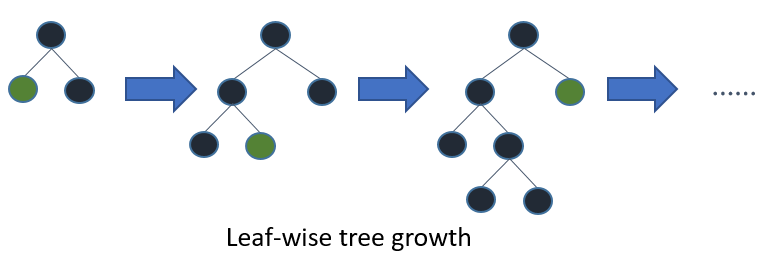
\includegraphics[width=\linewidth]{figures/lightgbm_leaf_wise.png}
    \\[1mm]\small (b) Phát triển cây theo lá tốt nhất
\end{minipage}
\caption{Minh họa hai chiến lược phát triển cây quyết định}
\label{fig:lightgbm-official-growth}
\caption*{\textit{Nguồn: Tài liệu chính thức của LightGBM \cite{lightgbm_docs}, giấy phép MIT; truy cập ngày 15/08/2026.}}
\end{figure}

Hình \ref{fig:lightgbm-official-growth} cho thấy sự khác biệt trực quan giữa hai chiến lược. Phương pháp theo tầng mở rộng đồng thời các nút ở cùng độ sâu và thường tạo ra cấu trúc tương đối cân đối. Ngược lại, LightGBM tiếp tục phân chia lá mang lại mức giảm hàm mất mát lớn nhất, vì vậy cây có thể phát triển không đối xứng. Cơ chế này góp phần nâng cao hiệu quả tối ưu, nhưng đồng thời đòi hỏi kiểm soát độ sâu và số lá để hạn chế hiện tượng quá khớp \cite{ke2017lightgbm,lightgbm_docs}.

\medskip
\noindent\textbf{CatBoost.}

CatBoost có khả năng xử lý trực tiếp biến phân loại và sử dụng cơ chế \textit{ordered boosting} để hạn chế rò rỉ thông tin trong quá trình huấn luyện \cite{prokhorenkova2018catboost}.

\section{Những thách thức khi mô hình hóa dữ liệu tín dụng}

\subsection{Thách thức đối với hiệu năng dự báo}

\noindent\textbf{Mất cân bằng lớp.}

\[
\mathcal{L}
=
-\sum_{i=1}^{N}
w_{y_i}
\sum_{k=1}^{K}
\mathbb{I}(y_i=k)\log p_{ik}.
\]
Trong đó $N$ là số quan sát; $K$ là số lớp; $w_{y_i}$ là trọng số gán cho lớp thật của quan sát $i$; $\mathbb{I}(y_i=k)$ bằng 1 khi $y_i=k$ và bằng 0 trong trường hợp khác; $p_{ik}$ là xác suất dự báo lớp $k$. Trọng số lớn hơn cho lớp hiếm làm sai số của lớp đó có ảnh hưởng lớn hơn tới hàm mất mát.

\medskip
\noindent\textbf{Tính thứ tự.}
Năm nhóm nợ có thứ tự rủi ro từ thấp đến cao nên hai sai số lệch một bậc và lệch bốn bậc không có mức độ nghiêm trọng như nhau. Luận văn sử dụng Ordinal MAE ở phần chỉ tiêu đánh giá để lượng hóa số bậc sai lệch trung bình; chỉ tiêu này chưa được hàm \mbox{\texttt{compute\_metrics()}} của mã nguồn báo cáo trong kết quả chính.

\subsection{Khả năng giải thích và yêu cầu ứng dụng}
\label{sec:shap-theory}

\[
f(\mathbf{x})=\phi_0+\sum_{j=1}^{p}\phi_j.
\]
Trong đó $f(\mathbf{x})$ là đầu ra mô hình cần giải thích; $\phi_0$ là giá trị nền; $p$ là số đặc trưng; và $\phi_j$ là đóng góp SHAP của đặc trưng $j$ cho hồ sơ $\mathbf{x}$ \cite{lundberg2017unified}.

\begin{figure}[H]
\centering
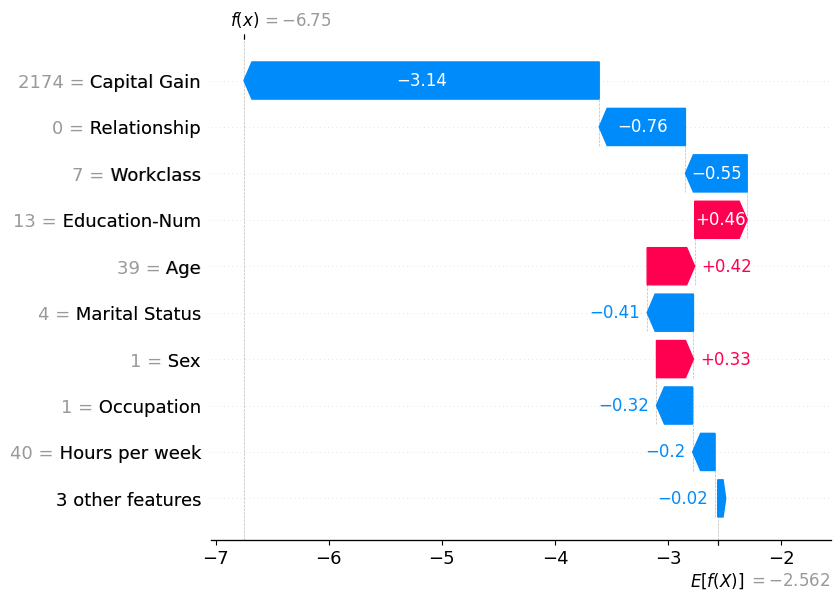
\includegraphics[width=0.72\textwidth]{figures/shap_waterfall_example.png}
\caption{Ví dụ biểu đồ waterfall minh họa nguyên lý phân rã dự báo theo giá trị SHAP}
\label{fig:shap-additive}
\caption*{\textit{Nguồn: Tài liệu chính thức của SHAP \cite{shap_docs}, giấy phép MIT, dựa trên phương pháp của Lundberg và Lee \cite{lundberg2017unified}; truy cập ngày 15/08/2026.}}
\end{figure}

Dự báo theo SHAP bắt đầu từ giá trị nền $\phi_0$ (ký hiệu $E[f(X)]$ trong Hình \ref{fig:shap-additive}), sau đó được điều chỉnh tăng hoặc giảm bởi đóng góp của từng đặc trưng cho tới khi đạt đầu ra $f(\mathbf{x})$ của hồ sơ đang xét. Dấu của $\phi_j$ cho biết chiều tác động đối với đầu ra đang được giải thích (thanh màu đỏ: đóng góp dương; thanh màu xanh: đóng góp âm), còn độ lớn tuyệt đối phản ánh cường độ đóng góp. Hình \ref{fig:shap-additive} chỉ minh họa nguyên lý phân rã từ tài liệu SHAP; các giá trị SHAP thực nghiệm của luận văn được tính riêng trên dữ liệu tín dụng ở Chương 4.

\begin{figure}[H]
\centering
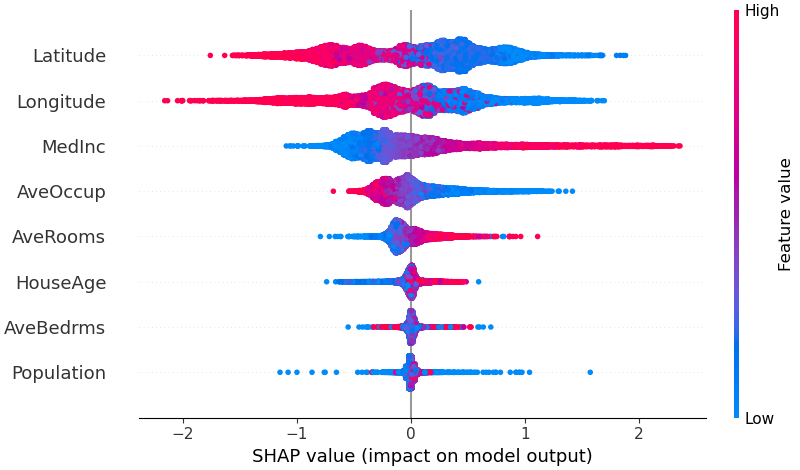
\includegraphics[width=0.82\textwidth]{figures/shap_beeswarm_example.png}
\caption{Ví dụ biểu đồ SHAP beeswarm trong phân tích mức độ tác động của đặc trưng}
\label{fig:shap-official-beeswarm}
\caption*{\textit{Nguồn: Kho tài liệu chính thức của SHAP \cite{shap_docs}, dựa trên phương pháp của Lundberg và Lee \cite{lundberg2017unified}, giấy phép MIT; truy cập ngày 15/08/2026.}}
\end{figure}

Trong biểu đồ beeswarm, mỗi điểm biểu thị một quan sát; vị trí trên trục hoành phản ánh giá trị SHAP, còn màu sắc thể hiện mức độ cao hoặc thấp của giá trị đặc trưng. Các đặc trưng được sắp xếp theo tổng độ lớn ảnh hưởng, qua đó cho phép xem xét đồng thời tầm quan trọng, chiều tác động và mức độ phân tán của ảnh hưởng trên toàn bộ tập dữ liệu. Hình \ref{fig:shap-official-beeswarm} chỉ minh họa cách đọc biểu đồ từ tài liệu SHAP; các kết luận thực nghiệm của luận văn được rút ra từ dữ liệu tín dụng và các biểu đồ được tạo riêng ở Chương 4.

\section{Hệ thống chỉ tiêu đánh giá mô hình}

\subsection{Chỉ tiêu tổng thể và theo lớp}

\noindent\textbf{Accuracy.}
\[
Accuracy=
\frac{\sum_{k=1}^{K}C_{kk}}
{\sum_{i=1}^{K}\sum_{j=1}^{K}C_{ij}}.
\]
Trong đó $C_{ij}$ là số quan sát có lớp thật $i$ và lớp dự báo $j$; tử số là tổng phần tử đường chéo; mẫu số là tổng số quan sát.

\medskip
\noindent\textbf{Precision, Recall và F1.}
\[
Precision_k=\frac{TP_k}{TP_k+FP_k},
\qquad
Recall_k=\frac{TP_k}{TP_k+FN_k},
\]
Trong đó $TP_k$ là số dự báo đúng lớp $k$; $FP_k$ là số quan sát lớp khác bị dự báo nhầm thành $k$; và $FN_k$ là số quan sát lớp $k$ bị dự báo sang lớp khác.
\[
F1_k=2\frac{Precision_k\times Recall_k}{Precision_k+Recall_k}.
\]

\subsection{Chỉ tiêu cho dữ liệu mất cân bằng}

\noindent\textbf{Macro F1.}
\[
F1_{\mathrm{macro}}=\frac{1}{K}\sum_{k=1}^{K}F1_k.
\]

\medskip
\noindent\textbf{Weighted F1.}
\[
F1_{\mathrm{weighted}}=\sum_{k=1}^{K}\frac{n_k}{N}F1_k.
\]
Trong đó $n_k$ là số quan sát thật của lớp $k$ và $N$ là tổng số quan sát. Khi một lớp chiếm tỷ trọng rất lớn, Weighted-F1 có thể che khuất hiệu năng thấp của lớp hiếm.

\medskip
\noindent\textbf{Balanced Accuracy.}
\[
Balanced\ Accuracy=\frac{1}{K}\sum_{k=1}^{K}Recall_k.
\]
Balanced Accuracy là trung bình Recall của $K$ lớp, nên mỗi lớp có trọng số như nhau bất kể tần suất.

\subsection{Chỉ tiêu phản ánh thứ tự nhóm nợ}

\noindent\textbf{Ordinal MAE.}
\[
Ordinal\ MAE=\frac{1}{N}\sum_{i=1}^{N}|y_i-\hat{y}_i|.
\]
Ký hiệu có ý nghĩa như phần Tính thứ tự; giá trị càng nhỏ thì khoảng cách nhóm dự báo so với nhóm thật càng thấp.

\section{Nghiên cứu liên quan, khoảng trống và định hướng}

\subsection{Kết quả chính của các nghiên cứu liên quan}

Hand và Henley \cite{hand1997statistical} hệ thống hóa các phương pháp phân loại thống kê; Thomas \cite{thomas2000survey} mở rộng phạm vi từ đánh giá tại thời điểm phê duyệt sang theo dõi hành vi trong vòng đời khoản vay. Baesens và cộng sự \cite{baesens2003benchmarking} và Lessmann và cộng sự \cite{lessmann2015benchmarking} cho thấy hiệu quả mô hình phụ thuộc vào dữ liệu, thước đo và quy trình đánh giá.

Brown và Mues \cite{brown2012experimental} nhấn mạnh ảnh hưởng của mất cân bằng. Xia và cộng sự \cite{xia2017boosted} cho thấy boosted tree có khả năng cải thiện dự báo. Barboza và cộng sự \cite{barboza2017machine} ghi nhận kết quả cạnh tranh của các mô hình cây trong dự báo phá sản. Dastile và cộng sự \cite{dastile2020statistical} chỉ ra các hạn chế phổ biến về dữ liệu nhỏ, mất cân bằng, thiếu chuẩn đánh giá và khả năng giải thích.

Tại Việt Nam, nghiên cứu thường tập trung vào đánh giá rủi ro tín dụng cá nhân, rủi ro doanh nghiệp và dự báo nợ xấu. Tuy nhiên, chưa có nhiều nghiên cứu công bố việc phân loại trực tiếp năm nhóm nợ trên dữ liệu thực tế, kết hợp so sánh nhiều mô hình, chia dữ liệu theo thời gian, đánh giá có xét thứ tự và phân tích khả năng giải thích.

\subsection{Khoảng trống và định hướng của luận văn}

\begin{enumerate}
    \item Phần lớn nghiên cứu dùng mục tiêu nhị phân.
    \item Tính thứ tự của năm nhóm nợ chưa được khai thác đầy đủ.
    \item Dữ liệu thực tế tại ngân hàng Việt Nam ít được công bố.
    \item Phương pháp chia mẫu ngẫu nhiên vẫn được sử dụng phổ biến hơn phương pháp chia mẫu theo thời gian.
    \item Lớp rủi ro cao ít quan sát nhưng chưa được đánh giá đầy đủ.
    \item Mô hình phức tạp thường thiếu khả năng giải thích.
\end{enumerate}

\medskip
\noindent\textbf{Định hướng nghiên cứu.}
Luận văn xây dựng bài toán phân loại năm nhóm nợ, kiểm tra và hình thành các đặc trưng nghiệp vụ, sử dụng Logistic Regression làm mô hình cơ sở để đối chiếu với các mô hình cây và mô hình tăng cường, đồng thời xử lý mất cân bằng lớp, đánh giá bằng hệ thống chỉ tiêu đa lớp và giải thích mô hình thông qua mức độ quan trọng của đặc trưng cùng SHAP. Thực nghiệm hiện tại sử dụng phép chia ngẫu nhiên có phân tầng; phép chia theo thời gian là yêu cầu cần thiết trong giai đoạn xây dựng nhãn chuyển nhóm nợ.

\section{Tóm tắt chương}

Chương này đã trình bày cơ sở lý thuyết, thành tựu và hạn chế của các công trình nền tảng, các mô hình được sử dụng, các vấn đề đặc thù của dữ liệu tín dụng, hệ thống chỉ tiêu đánh giá, tổng quan nghiên cứu, khoảng trống và định hướng của luận văn.

Trên cơ sở lý thuyết và định hướng đã xác lập, Chương 3 sẽ trình bày cụ thể nguồn dữ liệu, quy trình xử lý, phân tích khám phá dữ liệu, xây dựng đặc trưng nghiệp vụ và phương pháp thực nghiệm được cài đặt trong mã nguồn trên hai bộ dữ liệu thực tế của luận văn.
